\documentclass[aspectratio=169,unicode,dvipdfmx,14pt]{beamer}


\usepackage{url}
\usepackage{bm}
\usepackage{amsmath}
\usepackage{amssymb}
\usepackage{mathtools}
\usepackage{graphicx}
\usepackage[absolute,overlay]{textpos}
\usepackage{hyperref}
\usepackage{listings}
\usepackage{changepage}
\usepackage{lipsum}


\usefonttheme[onlymath]{serif}

\DeclareMathOperator*{\argmax}{argmax}

\DeclarePairedDelimiterX{\infdivx}[2]{(}{)}{%
  #1\;\delimsize\|\;#2%
}
\newcommand{\infdiv}{D_{\scriptsize \mbox{KL}}\infdivx}
\DeclarePairedDelimiter{\norm}{\lVert}{\rVert}

\hypersetup{
	setpagesize=false,
	bookmarksnumbered=true,%
	bookmarksopen=true,%
	colorlinks=true,%
	linkcolor=blue,
	citecolor=red,
}

\newcommand\FontMath{\fontsize{10}{12}\selectfont}
\renewcommand{\baselinestretch}{1.3}
\renewcommand{\familydefault}{\sfdefault}
\renewcommand{\kanjifamilydefault}{\gtdefault}
\usepackage[deluxe, expert]{otf}

\setbeamertemplate{navigation symbols}{}
\setbeamertemplate{footline}[frame number]
\setbeamerfont{footline}{size={\fontsize{15}{15}}}

\setbeamerfont{author}{size=\Large}
\setbeamerfont{institute}{size=\normalsize\itshape}
\setbeamerfont{title}{size=\huge}
\setbeamerfont{subtitle}{size=\LARGE\normalfont\slshape}


\title{PLSA}
\author{\texorpdfstring{正田 備也\newline\href{mailto:masada@rikkyo.ac.jp}{masada@rikkyo.ac.jp}}{正田 備也}}
\date{}

\begin{document}

\begin{frame}
\titlepage
\end{frame}

\section{混合多項分布の問題点}

\begin{frame}\frametitle{Contents}
\Large \tableofcontents[currentsection]
\end{frame}

\begin{frame}{混合多項分布}
\begin{itemize}
\item 混合多項分布モデルでは、例えば文書クラスタリングへの応用の場合、一つの文書がそれ全体で意味的なまとまりを持つと仮定することになる
\begin{itemize}
\item ニュース記事であれば、一つの記事まるごとが、特定のカテゴリ(ex. 政治、経済、スポーツ、etc)に割り振られる。
\end{itemize}
\item つまり、一つの文書内は意味的に均一だと、仮定している
\item しかし、この仮定は文書の実態に合わない
\item というのも、一つの文書は複数の話題を含みうるからである
\end{itemize}
\end{frame}

\begin{frame}{混合多項分布の改良としてのPLSA}
\begin{itemize}
\item 混合多項分布と同様、カテゴリの違いは、語彙集合上に定義された多項分布の違いとして表す
\begin{itemize}
\item 政治について書かれたテキストと、スポーツについて書いたテキストとでは、どの単語がどのくらいの確率で出現するかが異なる、という考え方。
\end{itemize}
\item 混合多項分布とは異なり、一つの文書に含まれる単語トークン群が、唯一の単語多項分布からではなく、\underline{複数の}単語多項分布から生成されると、仮定する→\underline{PLSAモデル}
\begin{itemize}
\item 同じ文書内に、異なる単語多項分布に由来する単語トークンが混ざっていてもよい、という考え方。
\item 同じ文書が複数の「トピック」を含みうる、という考え方。
\end{itemize}
\end{itemize}
\end{frame}

\begin{frame}{PLSA (probabilistic latent semantic analysis)}
\begin{itemize}
\item PLSI (probabilistic latent semantic indexing)とも呼ばれる
\item LSAの確率モデル版、ということ
\begin{itemize}
\item LSAは、単語-文書行列の特異値分解で次元圧縮する手法(後述)
\end{itemize}
\item 生成モデルとして記述すると…
\begin{itemize}
\item 文書に固有のトピック多項分布(その文書でどのトピックがどのくらい現れやすいか)から、単語トークン毎にトピックをdraw
\item そのトピックに対応する単語多項分布(そのトピックについて書くときどの単語がどのくらい使われやすいか)から単語をdraw
\end{itemize}

\end{itemize}

\end{frame}

\begin{frame}
\begin{figure}[htbp]
\begin{center}
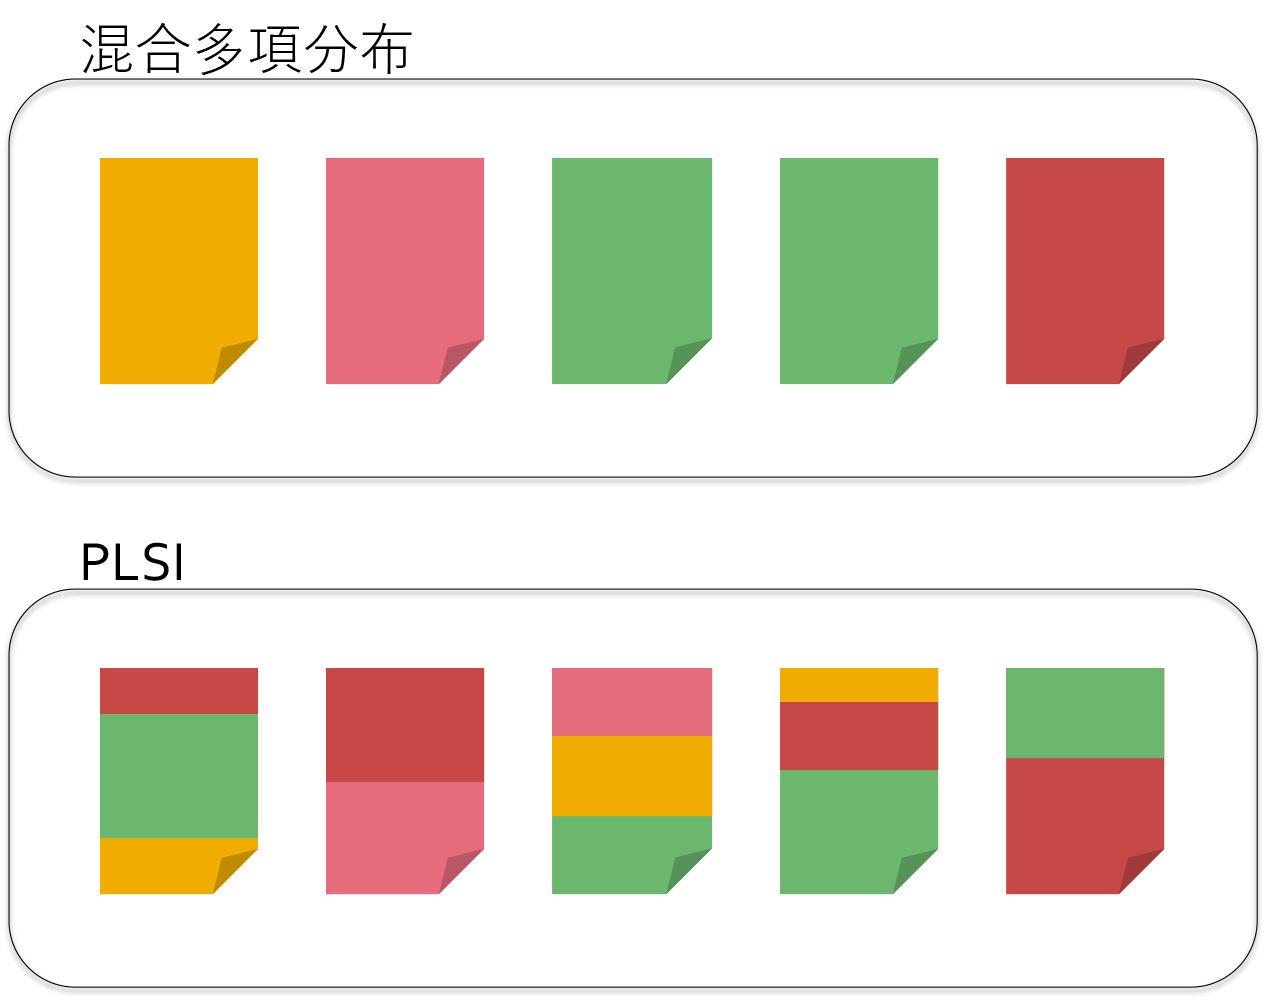
\includegraphics[scale=.21]{PLSI1.jpg}
\caption{混合多項分布とPLSAの違い}
\label{}
\end{center}
\end{figure}\end{frame}

\begin{frame}
\begin{figure}[htbp]
\begin{center}
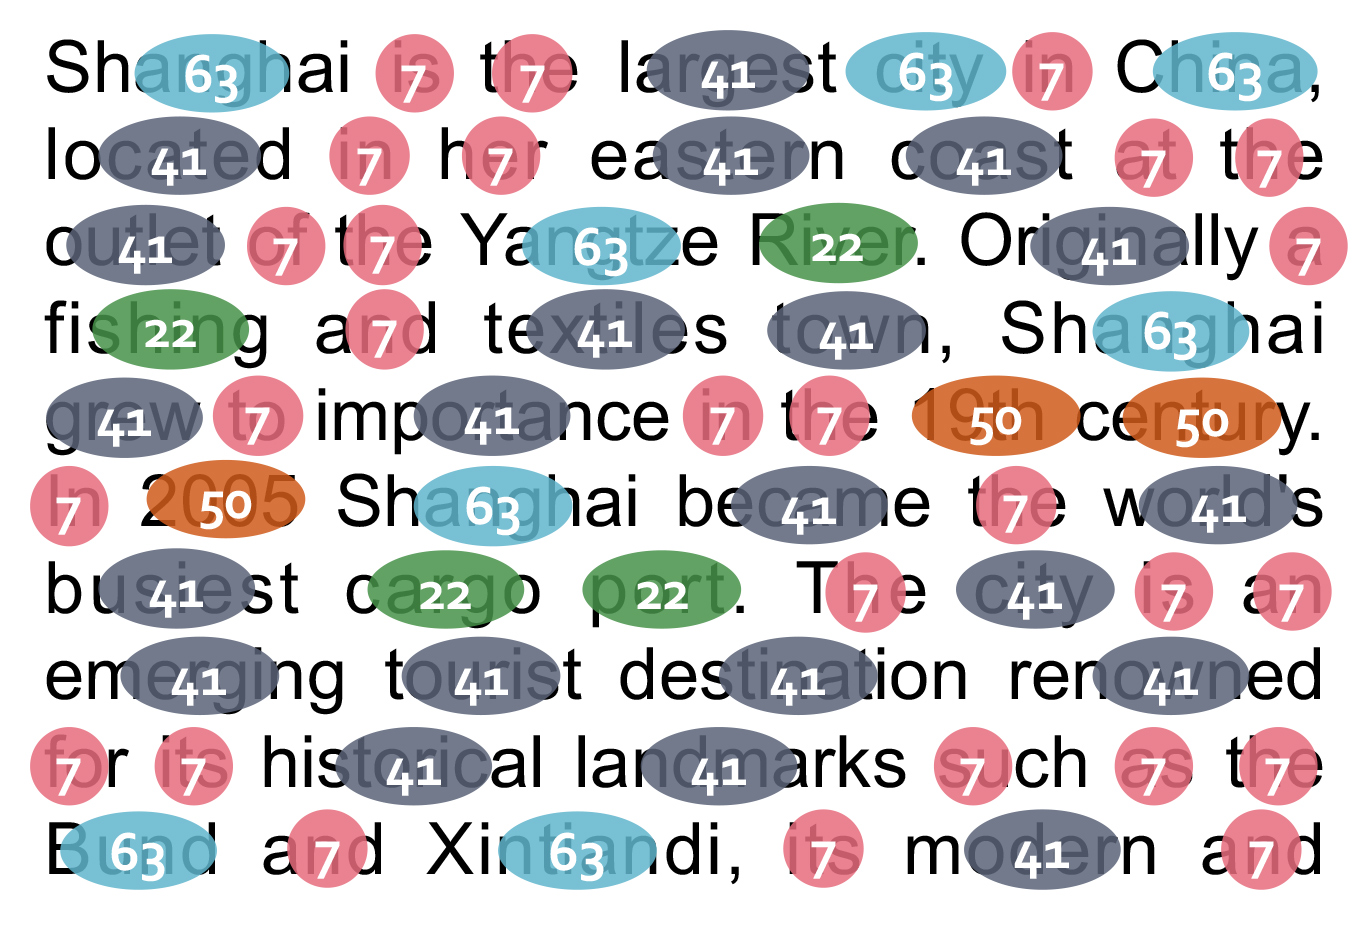
\includegraphics[scale=.22]{PLSI2.jpg}
\vspace{-.2in}
\caption{PLSAでは同じ文書の単語トークンが複数の単語多項分布に由来しうる}
\label{}
\end{center}
\end{figure}
\end{frame}

\section{PLSA (probabilistic latent semantic analysis)}

\begin{frame}\frametitle{Contents}
\Large \tableofcontents[currentsection]
\end{frame}

\begin{frame}{PLSA (probabilistic latent semantic analysis)}
\begin{itemize}
\item LSA(latent semantic analysis)をprobabilisticにしたモデル
\begin{itemize}
\item LSAについては次スライドの図を参照(実態は単なるSVD)
\end{itemize}
\item 同じ文書内でも、異なる単語トークンは、異なる単語多項分布から生成されうる(=異なるトピックを表現しうる)
\item どのトピックがどのくらいの確率で使われるかが、文書によって異なる
\item PLSAにおける単語多項分布を、トピック(topic)と呼ぶ
\begin{itemize}
\item 混合多項分布では、複数ある単語多項分布を、クラスタやコンポーネントと呼んでいた
\item PLSAは最もシンプルなトピックモデル
\end{itemize}
\end{itemize}
\end{frame}

\begin{frame}{LSAの概念図}
\FontMath
\vspace{-.2in}
\begin{figure}[htbp]
\begin{center}
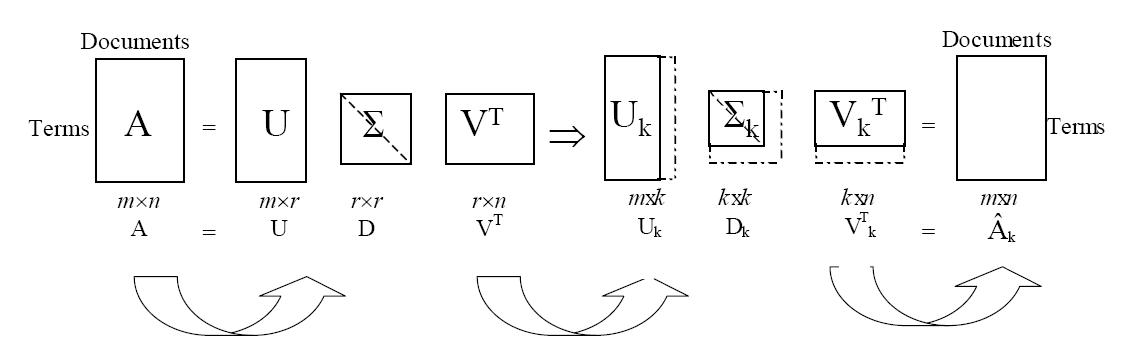
\includegraphics[scale=0.47]{svd1.jpg}
\caption{\href{https://liqiangguo.wordpress.com/2011/06/09/latent-semantic-analysis/}{LSAの概念図}}
\label{fig:LSA}
\end{center}
\end{figure}
\begin{itemize}
\item 左から順に、データ行列の特異値分解、低ランク近似、元のデータ行列の再現
\item $m$が語彙サイズ、$n$が文書数、$k$がトピック数($r$は元のデータ行列のランク)
\end{itemize}
\end{frame}

\begin{frame}{Notations}
\begin{itemize}
\item 語彙集合$\mathcal{V} = \{ 1, \ldots, W \}$ {\footnotesize(単語とそのindexを同一視することとする)}
\item トピック集合$\mathcal{T} = \{ 1, \ldots, K \}$ {\footnotesize(トピックとそのindexを同一視することとする)}
\item 文書集合$\mathcal{D} = \{ \bm{x}_1, \ldots, \bm{x}_D \}$
\item 文書$\bm{x}_d$の$i$番目に出現する単語を$x_{d,i}$という確率変数で表す
\item 文書$\bm{x}_d$の$i$番目に出現する単語が表現するトピックを$z_{d,i}$という確率変数で表す
\item $x_{d,i}$の値は観測されているが、$z_{d,i}$の値は観測されていない
\begin{itemize}
\item つまり、$z_{d,i}$は潜在変数。
\end{itemize}
\end{itemize}
\end{frame}


\begin{frame}{PLSAにおける同時分布}
\vspace{-.05in}
\begin{itemize}
\item PLSAでは、$x_{d,i}$がトピック$t_k$を表現し、かつそのトピックを表現するために現にその位置にある単語($v_w$とする)が使われる同時確率、つまり$p(x_{d,i} = w, z_{d,i} = k)$は
\begin{align}
p(x_{d,i} = w, z_{d,i} = k ) = p(x_{d,i} = w | z_{d,i}=k) p(z_{d,i}=k)
\end{align}
\item $p(z_{d,i}=k)$は、文書$\bm{x}_d$の$i$番目の単語が、他のトピックではなく、第$k$トピックを表現する確率
\item $p(x_{d,i} = w |z_{d,i}=k)$は、第$k$トピックを表現するときに、他の単語ではなく、第$w$単語が使われる確率
\item さらにPLSAでは以下のように仮定する(次スライド)
\end{itemize}
\end{frame}

\begin{frame}{PLSAにおいて仮定すること}
\begin{itemize}
\item どの$i,i^\prime$についても$p(z_{d,i}=k)=p(z_{d,i^\prime}=k)$と仮定する
\begin{itemize}
\item そこで、$p(z_{d,\cdot}=k)=\theta_{d,k}$とおく
\item 同じ文書内なら、どの単語トークンであれ、第$k$トピックを表現する確率は、同じ
(場所によってトピック確率が違ったりしない)
\end{itemize}
\item どの$d, d^\prime$や$i,i^\prime$についても、$p(x_{d,i}=w|z_{d,i}=k) = p(x_{d^\prime,i^\prime}=w|z_{d^\prime,i^\prime}=k)$と仮定する
\begin{itemize}
\item そこで、 $p(x_{\cdot,\cdot}=w|z_{\cdot,\cdot}=k)=\phi_{k,w}$とおく
\item 同じコーパス内なら、どの文書のどの単語トークンであれ、それが第$k$トピックを表現するために使われるならば(条件付き確率の条件の部分)、どの単語がどの確率で第$k$トピックを表現するかは、同じ
(単語確率分布とトピックが一対一に対応している)
\end{itemize}
\end{itemize}
\end{frame}

\begin{frame}{PLSAにおける観測データの尤度}
\FontMath
同時分布は
\vspace{-.1in}
\begin{align}
p(x_{d,i} = w, z_{d,i} = k ) & = p(x_{d,i} = w | z_{d,i}=k) p(z_{d,i}=k)
= \phi_{k,x_{d,i}} \theta_{d,k}
\end{align}
潜在変数を周辺化
\vspace{-.1in}
\begin{align}
p(x_{d,i}=v_w) & = \sum_{k=1}^K \phi_{k,x_{d,i}} \theta_{d,k}
\end{align}
各トークンの独立性の仮定より
\vspace{-.1in}
\begin{align}
p(\bm{x}_d) & = \prod_{i=1}^{N_d} \bigg( \sum_{k=1}^K \phi_{k, x_{d,i}} \theta_{d,k} \bigg)
\end{align}
各文書の独立性の仮定より
\begin{align}
p(\mathcal{D}) & = \prod_{d=1}^D \prod_{i=1}^{N_d} \bigg( \sum_{k=1}^K \phi_{k, x_{d,i}} \theta_{d,k} \bigg)
\end{align}
\end{frame}

\begin{frame}{混合多項分布とPLSAの比較}
\begin{itemize}
\item PLSAにおける$\bm{x}_d$の尤度
\begin{align}
p(\bm{x}_d) & = \prod_{i=1}^{N_d} \bigg( \sum_{k=1}^K \phi_{k, x_{d,i}} \theta_{d,k} \bigg)
\end{align}
\item 混合多項分布における$\bm{x}_d$の尤度
\begin{align}
p(\bm{x}_d) = \sum_{k=1}^K \theta_k \prod_{i=1}^{N_d} \phi_{k,x_{d,i}}
\end{align}
\end{itemize}
\end{frame}

\begin{frame}{Jensenの不等式の適用}
\FontMath
\vspace{-.15in}
\begin{align}
\ln p(\bm{x}_d) & = \ln \prod_{i=1}^{N_d} \bigg( \sum_{k=1}^K  \phi_{k, x_{d,i}} \theta_{d,k} \bigg)
\notag \\ & 
= \sum_{i=1}^{N_d} \ln \bigg( \sum_{k=1}^K q_{d,i,k} \frac{ \phi_{k, x_{d,i}} \theta_{d,k} }{ q_{d,i,k} } \bigg)
\notag \\
& \geq \sum_{i=1}^{N_d} \bigg( \sum_{k=1}^K q_{d,i,k} \ln \frac{ \phi_{k, x_{d,i}} \theta_{d,k} }{ q_{d,i,k} } \bigg)
\notag \\
& = \sum_{i=1}^{N_d} \sum_{k=1}^K q_{d,i,k} \ln ( \phi_{k, x_{d,i}} \theta_{d,k} )
- \sum_{i=1}^{N_d} \sum_{k=1}^K q_{d,i,k} \ln q_{d,i,k}
\notag \\
& = 
\sum_{i=1}^{N_d} \sum_{k=1}^K q_{d,i,k} \ln \phi_{k, x_{d,i}}
+ \sum_{i=1}^{N_d} \sum_{k=1}^K q_{d,i,k} \ln \theta_{d,k}
- \sum_{i=1}^{N_d} \sum_{k=1}^K q_{d,i,k} \ln q_{d,i,k}
\end{align}
where $\sum_{k=1}^K q_{d,i,k} = 1$ holds for all $d,i$.
\end{frame}

\begin{frame}{周辺尤度のlower bound}
\FontMath
\begin{align}
\ln p(\mathcal{D})
& \geq 
\sum_{d=1}^D \sum_{i=1}^{N_d} \sum_{k=1}^K q_{d,i,k} \ln \phi_{k, x_{d,i}} 
+ \sum_{d=1}^D \sum_{i=1}^{N_d} \sum_{k=1}^K q_{d,i,k} \ln \theta_{d,k}
- \sum_{d=1}^D \sum_{i=1}^{N_d} \sum_{k=1}^K q_{d,i,k} \ln q_{d,i,k}
\end{align}
最大化すべき目的関数は
\begin{align}
& \mathcal{L}(  \{ \bm{\theta}_d \}, \{ \bm{\phi}_k \}, \{ \bm{q}_{d,i} \} ) \notag \\
& = \sum_{d=1}^D \sum_{i=1}^{N_d} \sum_{k=1}^K q_{d,i,k} \ln \phi_{k, x_{d,i}} 
+ \sum_{d=1}^D \sum_{i=1}^{N_d} \sum_{k=1}^K q_{d,i,k} \ln \theta_{d,k}
- \sum_{d=1}^D \sum_{i=1}^{N_d} \sum_{k=1}^K q_{d,i,k} \ln q_{d,i,k}
\notag \\ & \mbox{ \ \ }
+ \sum_{d=1}^D \lambda_d \bigg( 1 - \sum_{k=1}^K \theta_{d,k} \bigg)
+ \sum_{k=1}^K \mu_k \bigg( 1 - \sum_{w=1}^W \phi_{k,w} \bigg)
+ \sum_{d=1}^D \sum_{i=1}^{N_d} \nu_{d,i} \bigg( 1 - \sum_{k=1}^K q_{d,i,k} \bigg)
\end{align}
\end{frame}

\begin{frame}{PLSAのEMアルゴリズム(1/2)}
\FontMath
M step
\begin{align}
\frac{\partial \mathcal{L}}{\partial \theta_{d,k}}
& = \sum_{i=1}^{N_d} \frac{ q_{d,i,k}  }{ \theta_{d,k} }
- \lambda_d \\
\therefore \theta_{d,k} & = \frac{ \sum_{i=1}^{N_d} q_{d,i,k} }{ \sum_{k=1}^K \sum_{i=1}^{N_d} q_{d,i,k} }
\end{align}
\begin{align}
\frac{\partial \mathcal{L}}{\partial \phi_{k,w}}
& = \frac{ \sum_{d=1}^D \sum_{i=1}^{N_d} \mathbbm{1}(x_{d,i} = w) q_{d,i,k} }{ \phi_{k, w} }
- \mu_k \\
\therefore \phi_{k,w} & 
= \frac{ \sum_{d=1}^D \sum_{i=1}^{N_d} \mathbbm{1}(x_{d,i} = w) q_{d,i,k} }
{ \sum_{w=1}^W \sum_{d=1}^D \sum_{i=1}^{N_d} \mathbbm{1}(x_{d,i} = w) q_{d,i,k} }
\notag \\ &
= \frac{ \sum_{d=1}^D \sum_{i=1}^{N_d} \mathbbm{1}(x_{d,i} = w) q_{d,i,k} }
{ \sum_{d=1}^D \sum_{i=1}^{N_d} q_{d,i,k} }
\end{align}
\end{frame}

\begin{frame}{PLSAのEMアルゴリズム(1/2)}
\FontMath
E step
\begin{align}
\frac{\partial \mathcal{L}}{\partial q_{d,i,k}}
& = \ln \phi_{k, x_{d,i}} + \ln \theta_{d,k} - \ln q_{d,i,k} - 1 - \nu_{d,i}
\\
\therefore q_{d,i,k} & \propto \phi_{k, x_{d,i}} \theta_{d,k}
\\
\therefore q_{d,i,k} & = \frac{ \phi_{k, x_{d,i}} \theta_{d,k} }{ \sum_{k=1}^K \phi_{k, x_{d,i}} \theta_{d,k} }
\end{align}
$x_{d,i} = x_{d,i^\prime}$ならば$q_{d,i,k} = q_{d,i^\prime,k}$となる。
つまり、PLSAでは同一文書内で別の場所に現れる同じ単語を区別できない。
よって、第$d$文書での第$w$単語のTFを$n_{d,w}$とすると
\begin{align}
q_{d,w,k} & = \frac{ \phi_{k, w} \theta_{d,k} }{ \sum_{k=1}^K \phi_{k, w} \theta_{d,k} }
\end{align}
\begin{align}
\theta_{d,k} = \frac{ \sum_{w=1}^W n_{d,w} q_{d,w,k} }{ \sum_{k=1}^K \sum_{w=1}^W n_{d,w} q_{d,w,k} }
\mbox{ , \ }
\phi_{k,w} 
= \frac{ \sum_{d=1}^D n_{d,w} q_{d,w,k} }
{ \sum_{w=1}^W \sum_{d=1}^D n_{d,w} q_{d,w,k} }
\end{align}
\end{frame}


\end{document}